\documentclass[10pt,unicode]{beamer}
%\documentclass[10pt,aspectratio=169,unicode]{beamer}

%% 日本語
\usepackage{luatexja}

%% 作図用パッケージ
%% [TikZ & PGF のマニュアル](https://www.ctan.org/pkg/pgf)
\usepackage{graphicx,xcolor}
\usepackage{tikz}
\usetikzlibrary{cd}
\tikzset{ ampersand replacement=\& }

%% 画像を手軽に透過する
\usepackage{transparent}

%% 位置調整用パッケージ
\usepackage[absolute,overlay]{textpos}
\usepackage{adjustbox}
\usepackage{multicol}

%% 画像フォルダ指定
\graphicspath{{./images}}

%% beamerのテーマの設定
%% [Beamerのマニュアル](https://ctan.org/pkg/beamer)
\usetheme{CambridgeUS}
%\usecolortheme{dolphin}
\usefonttheme{professionalfonts}

%% 目次の節番号の設定
\setbeamertemplate{section in toc}[sections numbered]
\setbeamertemplate{subsection in toc}[subsections numbered]

%% 箇条書きの設定
%% [参考](https://ayapin-film.sakura.ne.jp/LaTeX/Slides/guide4beamer.pdf)
\setbeamertemplate{itemize items}[circle]
\setbeamertemplate{enumerate items}[default]

%% フォント指定(必ずbeamerテーマ設定の後)
\usepackage[haranoaji,deluxe,nfssonly,jis2004]{luatexja-preset}
\usepackage{luatexja-fontspec}
% 欧文フォント (順に rm,sf,tt)
\setmainfont[Ligatures=TeX]{TeXGyreTermes}
\setsansfont[Ligatures=TeX]{TeXGyreHeros}
\setmonofont[Ligatures=TeX]{Inconsolatazi4}
% 日本語フォント (順に rm,sf,tt)
\setmainjfont[BoldFont=HaranoAjiMincho-Bold]{HaranoAjiMincho-Regular}
\setsansjfont[BoldFont=HaranoAjiGothic-Medium]{HaranoAjiGothic-Regular}
%\setmonojfont[Ligatures=TeX]{Inconsolatazi4}

% ギリシャ語などのスペース調整
\ltjsetparameter{jacharrange={-2,-3,-8}}

%% 和文の既定フォントをゴシック体に変更
\renewcommand{\kanjifamilydefault}{\gtdefault}

%% 非表示要素を透過
\setbeamercovered{transparent=30}

%% ナビゲーションバー(右下の灰色のやつ)を消す
\setbeamertemplate{navigation symbols}{}

%% enumerate環境の番号定義を簡単にする
\usepackage{enumerate}

%% ルビ
%% \ruby{塩}{しお}, \ruby{味噌}{み|そ}, \ruby[g]{杜鵑}{ほととぎす}
%% [参考](https://qiita.com/zr_tex8r/items/42466cbcbeb670a3a2dc)
\usepackage{pxrubrica}

%% AMS関連と数学記号
\usepackage{amsmath}
\usepackage{amsfonts}
\usepackage{amssymb}
\usepackage{amscd}
\usepackage{mathrsfs}
\usepackage{mathtools}

%%--amsthm(定理の設定)
\usepackage{amsthm}
\newtheoremstyle{mystyle}%   % 定理スタイル名
    {}%                      % 上のスペース
    {}%                      % 下のスペース
    {\normalfont}%           % 定理内でのフォント
    {}%                      % インデント
    {\gtfamily\bfseries}%    % 定理の見出しフォント(証明の見出しは別で指定)
    {}%                      % 定理見出し後の文字
    {0.5em}%                 % 見出し後の空白
    {}%                      % 見出しの書式( \thmname{#1}\thmnumber{ #2}\thmnote{ (#3)} など)
\theoremstyle{mystyle}
\newtheorem{thm}{定理}[section]
\newtheorem{dfn}[thm]{定義}
\newtheorem{sym}[thm]{記号}
\newtheorem{cor}[thm]{系}
\newtheorem{lem}[thm]{補題}
\newtheorem{prop}[thm]{命題}
\newtheorem{eg}[thm]{例}
\renewcommand{\proofname}{\gtfamily\bfseries 証明\,}
%%--end_of_amsthm

%% 参考文献
%\bibliographystyle{jplain} % アルファベット順
\bibliographystyle{junsrt} % 引用順
\setbeamertemplate{bibliography item}[text]

%% URL を \url{ ~ } で書ける. リンクの色は印刷用に消している.
%% (その他のパッケージが読み込まれたか確認するので, なるべく後ろで読み込む)
%% bookmark は, hyperrefを含む. xurl は, 長いリンクを快適にするパッケージ.
\usepackage{bookmark}
\usepackage{xurl}
\hypersetup{unicode,bookmarksnumbered=true,hidelinks,final}

%% タイトル
\title[title CambridgeUS]{
  CambridgeUS のシンプル設定
}
\subtitle{
  ロゴも入る
}
\author[お名前]{あなたのお名前\inst{1}}
\institute[所属]{\inst{1}所属している団体名(1人なら\texttt{\textbackslash inst\{1\}}は不要)}
\date[日付]{発表する研究集会情報や日付など}

\titlegraphic{\flushright%
  %\transparent{0.4}%
  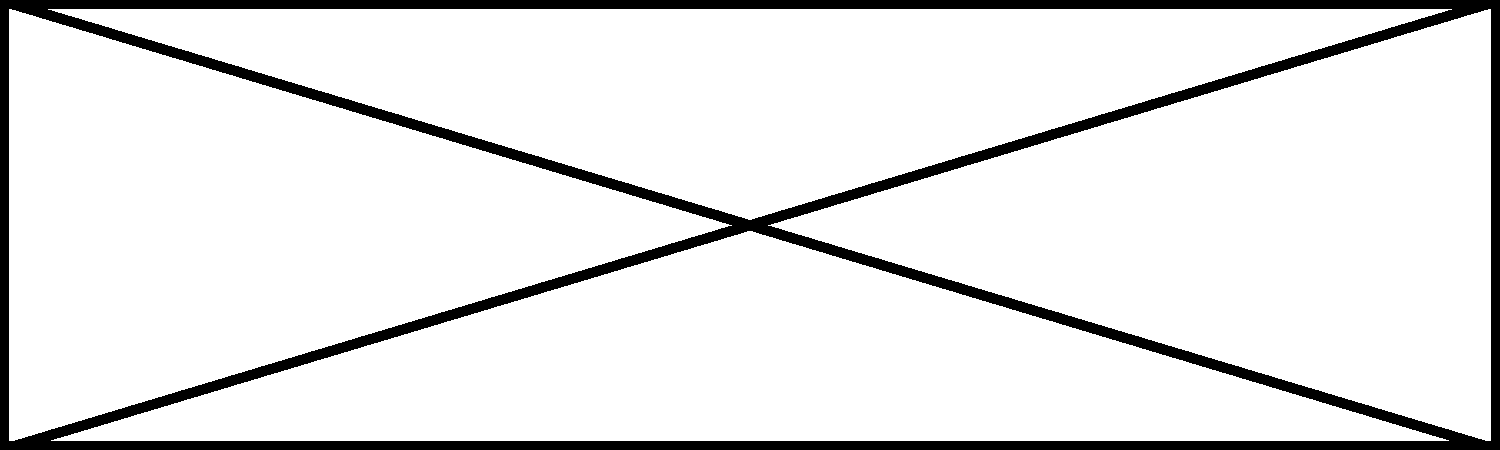
\includegraphics[height=0.1\pageheight]{dummy_logo_black.png}%
}


%% 節先頭毎に目次を追加
\AtBeginSection[]{
  \begin{frame}[noframenumbering,plain]{\insertsectionhead}{}
    \tableofcontents[currentsection]
  \end{frame}
}

%% ここから本文
\begin{document}
  %% タイトル
  \begin{frame}[noframenumbering,plain]{}{}
    \titlepage
  \end{frame}

  %% 目次
  \begin{frame}[noframenumbering,plain]{目次}{}
    \tableofcontents%[hideallsubsections]
  \end{frame}

  \section{最初の節}
  \begin{frame}{はじめの1歩}
    Beamer で作った PDF は, 全画面表示やプレゼンモードで使っていく.
    詰め込まないようにした方が綺麗に見える.
    詰め込むときは, 図示や{\scriptsize 文字サイズ}など工夫した方が良い.
    聴講者や発表会場によっても文字サイズは変わってくるかもしれない.

    \[
      \begin{tikzcd} % & を\& にすること!
        \mathscr{A} \arrow[d]\arrow[rd,"\iota_\mathscr{A}^{}"]\\
        \mathscr{D}b \arrow[r,"\iota_{\mathscr{D}b}^{}"] \& \mathscr{B}.
      \end{tikzcd}
    \]

    \pause % より詳細な設定ができる\only,\uncover,\visibleなどもある
    \begin{dfn}[定義の名前 \ast 無くてもよい]
      任意の$a\in\mathbb{R}$に対して, 次が成り立つ.
      \[
        a^2 \geq 0.
      \]
    \end{dfn}

    \vspace{1.2em} % 1.2 文字分 縦に 隙間を追加. マイナスもできる. 前に区切り文字を入れないとたまにおかしくなる.
    より詳しくは\,
    参考になる文献\footnote[1]{\cite{book:dummy}著者. 本のタイトル. 出版社, 出版年1900.}
    を参照.
  \end{frame}

  \section{次の節}
  \begin{frame}{その他の色確認}{}
    \begin{columns}
      \begin{column}[t]{0.5\textwidth-0.01\textwidth}
        箇条書き(\texttt{\textbackslash itemize})
        \begin{itemize}
          \item 最初
          \item 真ん中
          \item 最後
        \end{itemize}
      \end{column}
      \begin{column}[t]{0.5\textwidth-0.01\textwidth}
        \ruby{箇条}{か|じょう}書き(\texttt{\textbackslash enumerate})
        \begin{enumerate}[(i)]
          \item 最初
          \item 真ん中
          \item 最後
        \end{enumerate}
      \end{column}
    \end{columns}
  
    \begin{block}{block title}
      block body
    \end{block}
    \begin{alertblock}{alertblock title}
      alertblock body
    \end{alertblock}
    \begin{exampleblock}{exampleblock title}
      exampleblock body
    \end{exampleblock}
  \end{frame}

  %% 参考文献
  \section*{参考文献}
  \begin{frame}[noframenumbering,plain]{参考文献}{}
    \bibliography{ref}
  \end{frame}
\end{document}